%文責:中塚・黒崎

\subsection{CIB}
\subsubsection{基本設計思想}
CIB(Communication and Inhibit Board)は,イプシロンロケット搭載のためのシステム安全要求(電源のインヒビット機能)を満たすこと,および消費電力の高い5.8GHz送信機の電源系統を別とすることを目的として新規開発を行った基板であり,バッテリとEPSの間に挿入されている.また,VHF/UHFの受信機(RX)/送信機(TX)(西無線301A型)のためのマイコンであるRXPIC(PIC 16F877A),TXPIC(PIC 16F886)およびモデム回路もCIB上に搭載されている.RXPICはメインOBCより上位にあるものと考え,メインOBCを監視する.RXPIC及びTXPICはWDT(Watch Dog Timer)を用いて異常時には自身へリセットをかける.

\subsubsection{WDT回路}
タイマーIC SA555を二つ組み合わせることによってWDTをタイムアウトモード(一定期間内にMCUからの信号入力が無い場合,MCUを異常状態とみなしリセット信号を出力するモード)で搭載した.図\ref{fig:wdt}にその回路図を示す.

\begin{figure}[htbp]
	\centering
	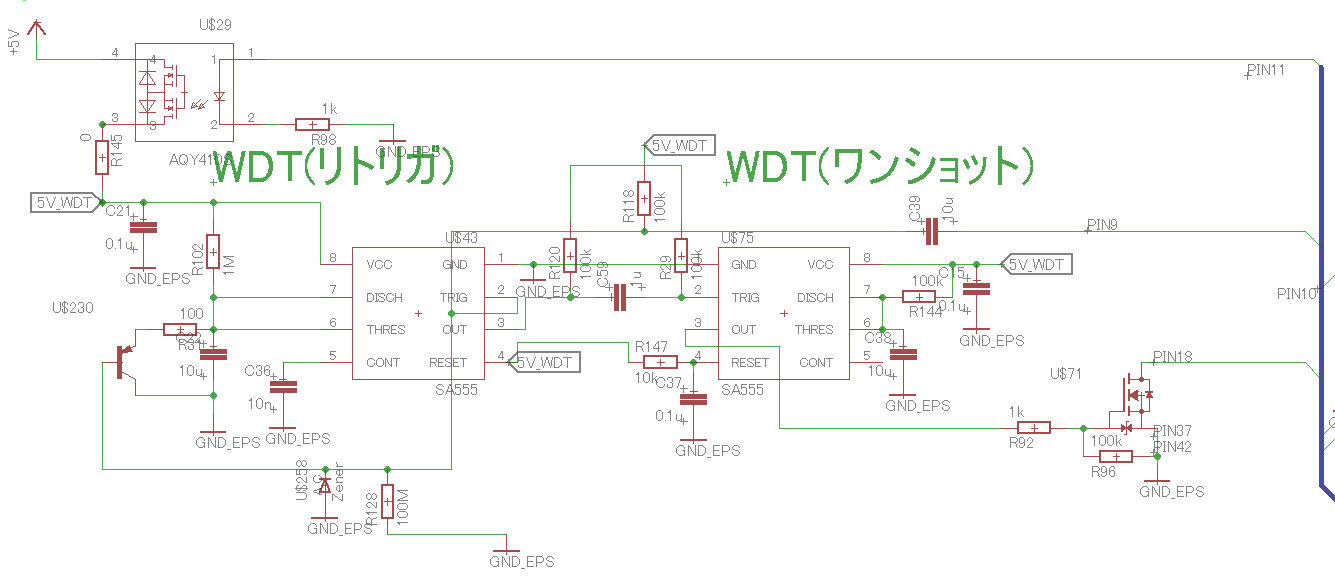
\includegraphics[width=\linewidth]{03/fig/wdt.png}
	\caption{WDT回路図}
	\label{fig:wdt}
\end{figure}

前段はMissing-Pulse Detectorとして機能させ,一定時間lowのパルスがMCU(今回はPIC)から送られてこない場合に,再びlowが来るまでOUTピンからlowを出力する.
後段はMono-stable Operationとして機能し,前段からのlow信号が入力されたら一定時間highを出力する.
これら二つ組み合わせることによって,MCUからLowがある一定秒送られなかった(MCUが動作停止した)場合に,後段がまた別の一定秒High信号を送ることができる.後段のOUTピンによってPICのMCLRを一定時間GNDに落とし復帰させればPICのリセットがかかる.

前段のTRIGピンがプルアップされているのは,MCUからの信号がlowで固定されてしまった故障モードにおいても次第にhighにすることでエラーを検知するためである.


\subsubsection{プログラム概要}
\paragraph{RXPIC役割}\label{par:RXPIC役割}
RXPICの持つ主要機能は大きく分けて以下のものがある.RXPICの各機能詳細は\ref{subsubsec:RXPIC詳細}参照.
\begin{itemize}
	\item 初期運用
	\item EPSリセット
	\item 無線機の周波数設定
	\item バッテリ電圧測定及び衛星モード切替
	\item アップリンクコマンド処理
\end{itemize}

\paragraph{TXPIC役割}\label{par:TXPIC役割}
TXPICの持つ主要機能は大きく分けて以下のものがある.TXPICの各機能詳細は\ref{subsubsec:TXPIC詳細}参照.
\begin{itemize}
	\item 初期運用
	\item ADCの値を取得
	\item レシーブコマンドダウンリンク
	\item CWダウンリンク(HKデータ/指定データ)
	\item FMダウンリンク(HKデータ/指定データ)
	\item スイッチ操作
\end{itemize}

\subsubsection{RXPIC詳細}\label{subsubsec:RXPIC詳細}
RXPICのフローチャートを図\ref{fig:3-4-2-1}に示す.
\begin{figure}[H]
	\centering
	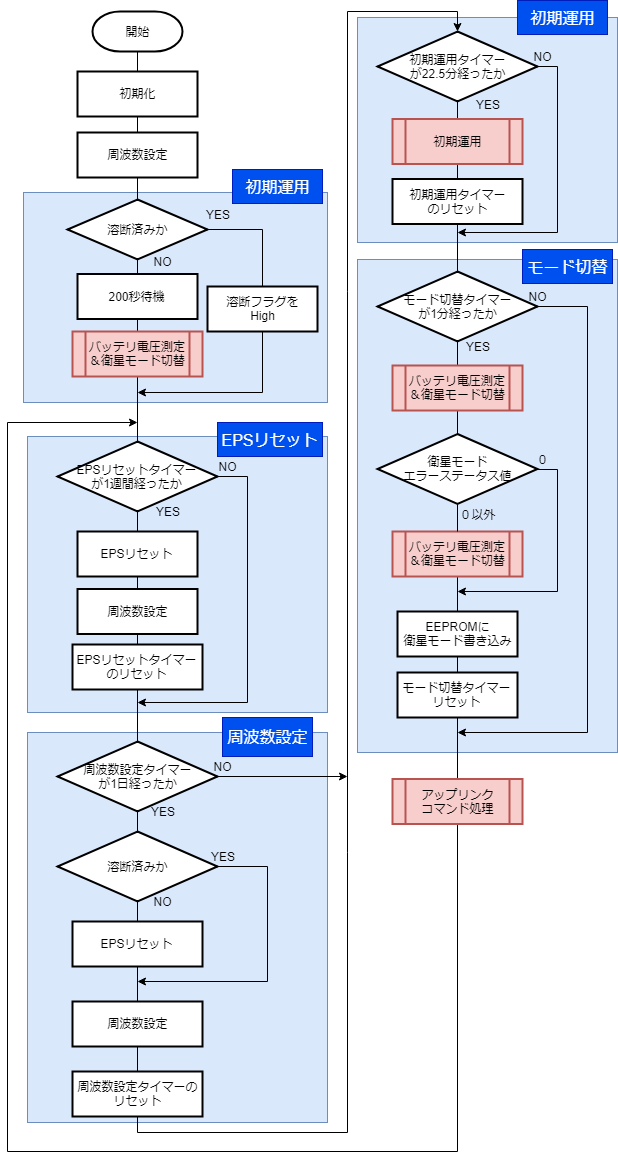
\includegraphics[scale=0.5]{03/fig/3-4-2-1.png}
	\caption{RXPIC全体フローチャート}
	\label{fig:3-4-2-1}
\end{figure}
以下でRXPICの各機能について説明する.
\paragraph{初期運用}
詳細については初期運用項(統合時ラベル付けして参照)を参照.

\paragraph{EPSリセット}
RXPICでは1週間毎にEPSリセットのタイマー割込みが発生する.これはRXPIC及びTXPIC以外の,EPSから電源供給されているコンポーネントの不具合が生じ,実装しているエラー処理で対応しきれないケースに備え,1週間毎にリセットをかけることを目的として実装した機能である.なお初期運用中は,これに加えて1日毎のEPSリセットも行われる.

\paragraph{無線機の周波数設定}
RXPICでは1日毎に無線機の周波数設定のタイマー割込みが発生する.無線機の周波数設定でエラーが生じ通信できなくなるケースに備え,通常の無線機の電源ON/OFFに伴う周波数設定とは別に実装した機能である.

\paragraph{バッテリ電圧測定及び衛星モード切替}
RXPICでは1分毎にバッテリ電圧測定及び衛星モード切替のためのタイマー割込みが発生する.バッテリ電圧に応じて衛星モードはNominal,Saving,Survivalに切り替わり,モードに応じてアクティブなコンポーネントが変化する.モード切替の概念を図\ref{fig:3-4-2-2}に示す.モード切替の閾値電圧の初期値はそれぞれ図\ref{fig:3-4-2-2}に示す値であり,これらの閾値はコマンドにより変更することができる.電圧降下時と上昇時の初期閾値電圧に差があるのは,電圧上昇によるモード切替に伴いアクティブなコンポーネントが増えることで一時的に電圧が降下し,直後に再びモード切替が起こることを防ぐためである.
\begin{figure}[H]
	\centering
	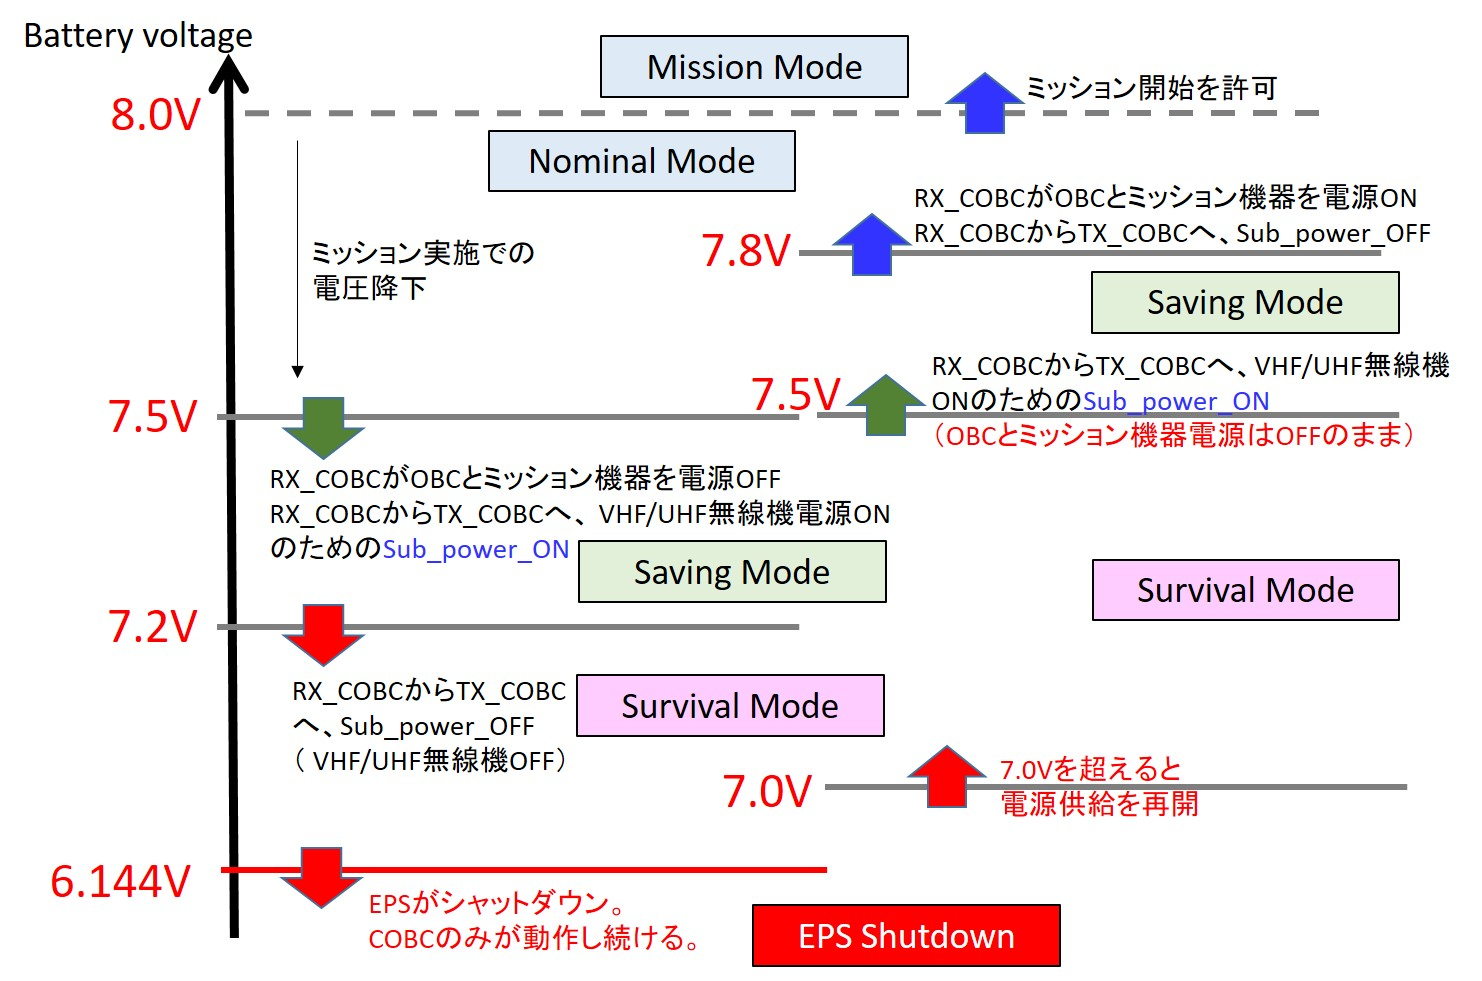
\includegraphics[scale=0.6]{03/fig/3-4-2-2.jpg}
	\caption{モード切替の概念図}
	\label{fig:3-4-2-2}
\end{figure}
バッテリ電圧測定及び衛星モード切替のフローチャートを図\ref{fig:3-4-2-3}に示す.
衛星モード切替では,バッテリー電圧,閾値電圧,及び前の衛星モードを取得し,それを元に切替処理を行っている.閾値電圧はメイン/サブEEPROMを,前の衛星モードはメイン/サブEEPROM及びグローバル変数を利用して,取得できないリスクを低減させている.また衛星モード切替中にエラーが生じ,正常に処理が完了できない場合には基本的にSavingモードに切り替える.
バッテリ電圧測定及び衛星モード切替処理では返り値として1byteのエラーステータスを用意しており,異なる2bitずつを異なるエラーに割り当てることで,同時に生じる複数のエラーを検知できるように実装している.1bitずつの割り当てでないのは,放射線等によるbit反転の影響を小さくするためである.エラー値の詳細についてはOP-S1-0109「CW通信フォーマット」の衛星モードエラーステータスを参照.また衛星モード切替の詳細については,OP-S1-0104「OrigamiSat-1 モード切替について」を参照.
\begin{figure}[H]
	\centering
	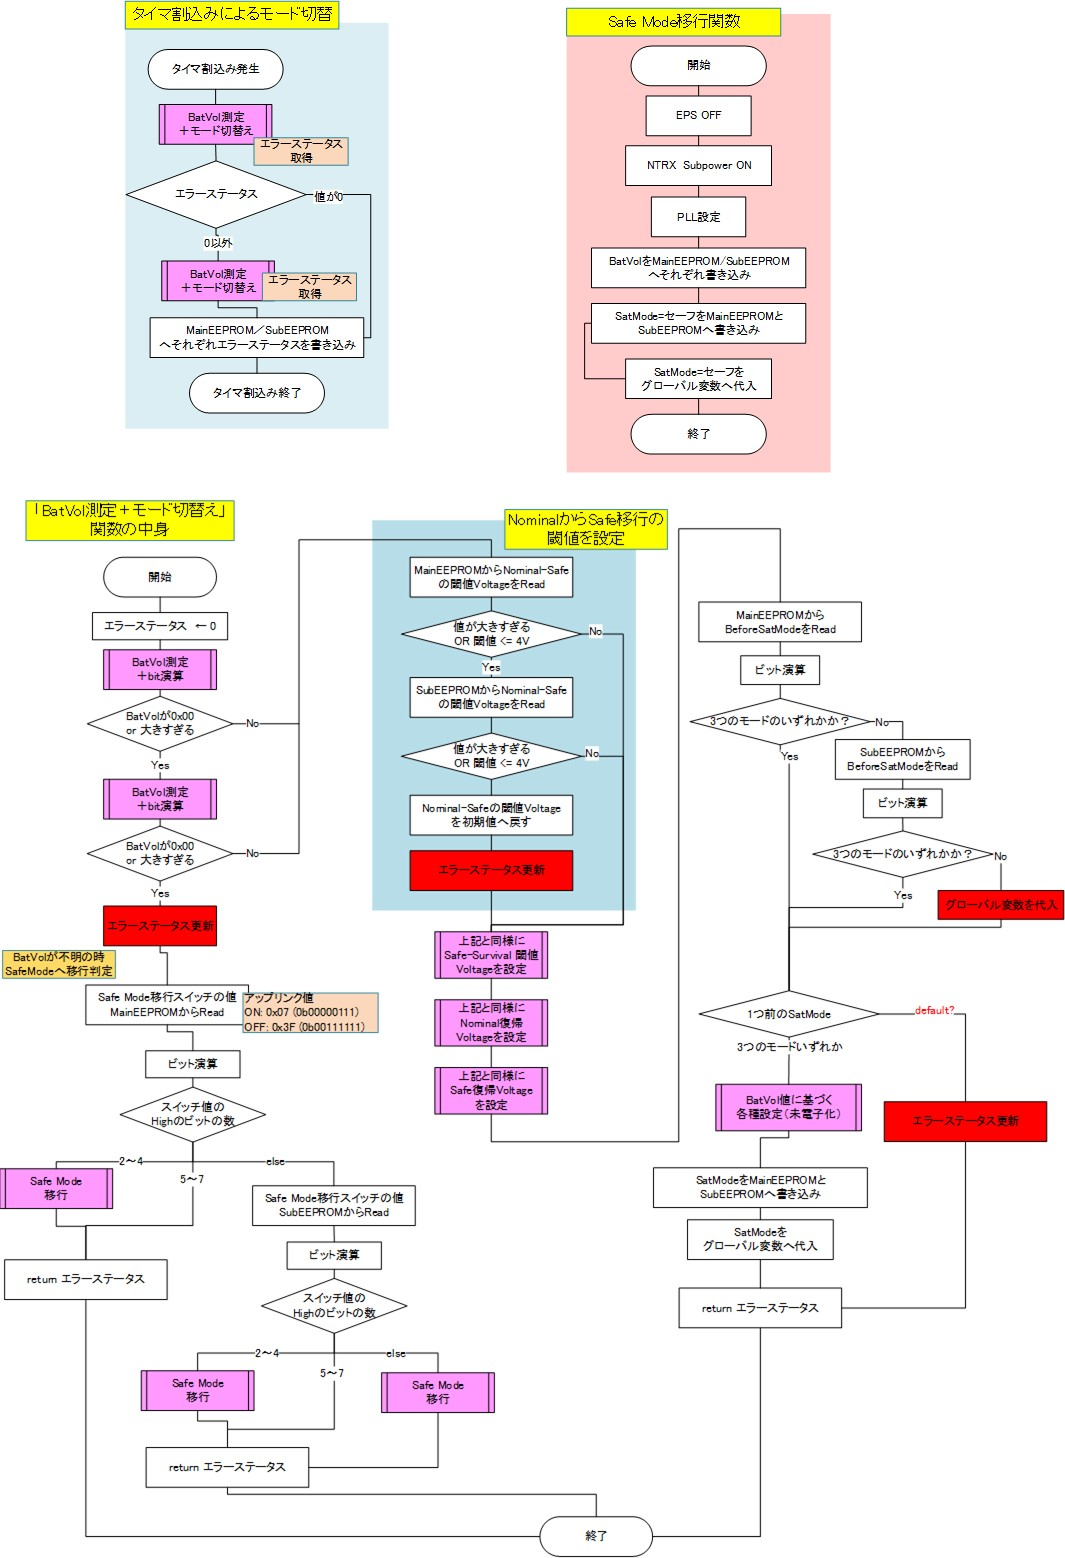
\includegraphics[scale=0.9]{03/fig/3-4-2-3.jpg}
	\caption{モード切替フローチャート}
	\label{fig:3-4-2-3}
\end{figure}

\paragraph{アップリンクコマンド処理}
RXPICのアップリンクコマンド処理時のフローチャートを図\ref{fig:3-4-2-4}に示す.地上局からのアップリンクコマンドを受信後コマンドIDの確認を行い,最終実行コマンドIDと同じであればコマンドの実行は行わない.これは地上局から誤って同じコマンドを2回送った時,衛星がそれを実行しないようにするためである.コマンドIDのチェックが終わった後はEEPROMにコマンドを書き込み,コマンドターゲットに応じて処理を行う.コマンドターゲットがRXPICであった場合のコマンド実行関数内では,コマンドタイプに応じてswitch文で分岐し,それぞれの処理を行っている.
\begin{figure}[H]
	\centering
	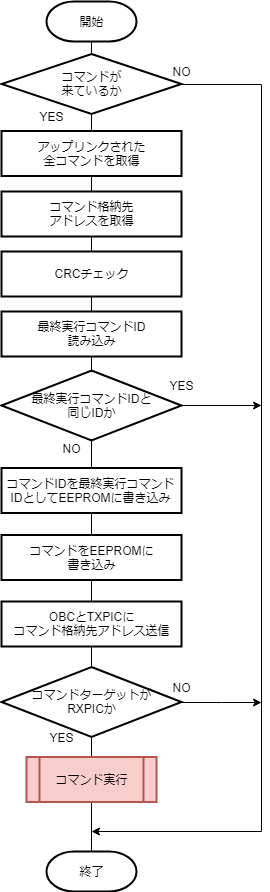
\includegraphics[scale=0.6]{03/fig/3-4-2-4.png}
	\caption{アップリンクコマンド処理フローチャート}
	\label{fig:3-4-2-4}
\end{figure}

\subsubsection{TXPIC詳細}\label{subsubsec:TXPIC詳細}
TXPICのフローチャートを図\ref{fig:3-4-2-5}に示す.図\ref{fig:3-4-2-5}のフローチャートとは別に割込み関数として,コマンドが来た際に
\ref{par:TXPIC役割}の主要機能のうち,レシーブコマンドダウンリンク,CWダウンリンク(データ),FMダウンリンク(HK/データ),スイッチ切替は,図\ref{fig:3-4-2-5}中のコマンド実行関数内で行われる.
\begin{figure}[H]
	\centering
	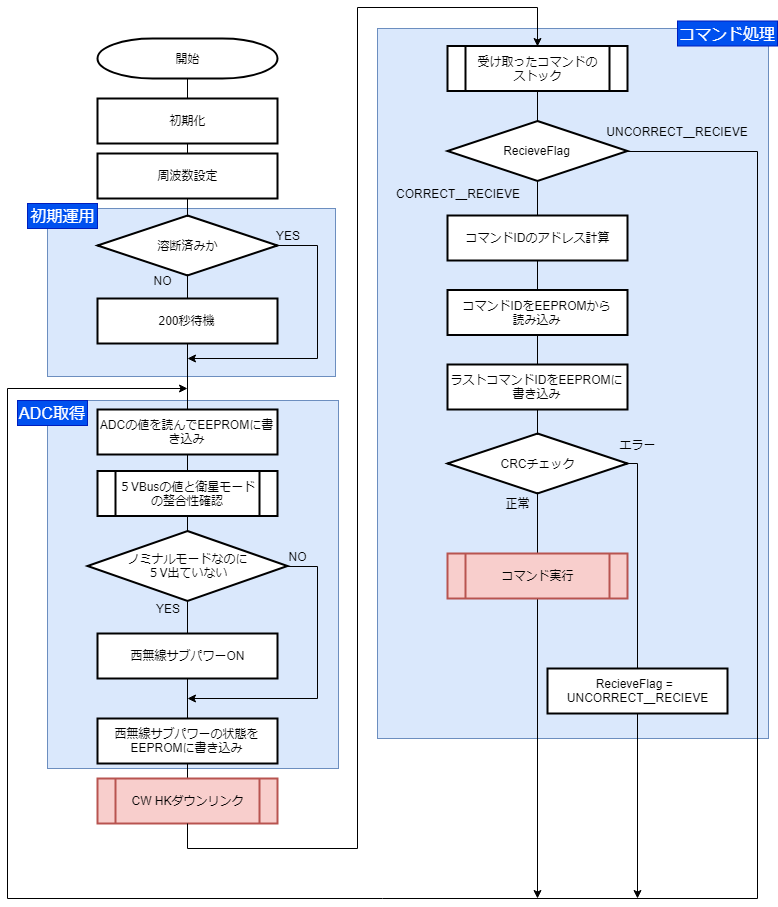
\includegraphics[scale=0.6]{03/fig/3-4-2-5.png}
	\caption{TXPIC全体フローチャート}
	\label{fig:3-4-2-5}
\end{figure}
以下でTXPICの各機能について説明する.

\paragraph{初期運用}
詳細については初期運用項(統合時ラベル付けして参照)を参照.

\paragraph{ADCの値を取得}
ADCのCH1-4の値を取得し,EEPROMに保存する.なお,CH1-4はそれぞれバッテリ温度,EPS5Vライン電圧,EPS3.3Vライン電圧,5Vライン電圧電圧の値を示す.ADCの値を取得後,EEPROMから衛星モードの読み込みを行い整合性を確認する.整合性がとれない,すなわちノミナルモードにもかかわらずEPS5Vラインの電圧が低かった場合,西無線のサブパワーをONにする.これは,ノミナル時にエラー等により西無線の電源が遮断され,地上局との通信ができなくなるリスクの低減のために実装を行った.

\paragraph{レシーブコマンドダウンリンク}
地上局からアップリンクされたコマンドを受信した後,RXPICからの指示を受けてTXPICはアップリンクされたコマンドを地上局に返す.
これはコマンドアップリンク時,衛星側がコマンドを受け取ったかどうか判断するために実装を行った.

\paragraph{CW ダウンリンク}
CWダウンリンクは,HKダウンリンクとコマンドによる指定データのダウンリンクの2種類がある.
CWHKダウンリンクフォーマットの詳細については,OP-S1-0109「CW通信フォーマット」を参照.
コマンドによる指定データのダウンリンクでは,コマンドによって指定されたEEPROMアドレスのデータを指定回数ダウンリンクする.CWによるデータダウンリンク機能は,FM及び5.8GHzデータ送信機能が共に失われた場合に備え実装を行った.

\paragraph{FMダウンリンク}
FMダウンリンクは,HKダウンリンクとコマンドによる指定データのダウンリンクの2種類がある.
FMダウンリンクフォーマットの詳細については,OP-S1-0108「FMダウンリンクフォーマット」を参照.

\paragraph{スイッチ切替}
コマンドに応じてヒーター,送受信機,5.8GHz送信機予備電源,溶断回路,WDT,FMPTT,CWKEYのON/OFFを切り替える.コマンドで時間を指定することにより,指定時間ON/OFFを切り替えた後,元の状態に戻す機能が実装されている.

\subsubsection{コメントや次回への改善点}
\begin{itemize}
	\item システム設計を早い時期にしっかり行い,優先順位の高いものからプログラムを作っていくべきだった.複数個所で使う重要な機能の開発が後半に残っていたことがあった.また,機能を実装したものの結局使わないものや,ほぼ同じ機能を持つ関数が複数存在する事態が開発途中で発生した.またOrigamiSat-1のCIBでは開発の遅れからエラー処理を実装しきれないところが多かった.システム設計を早期にしっかり行い,エラーについても体系的に処理を行いHKデータ等でダウンリンクすることで,エラー箇所の切り分けを行うことができれば故障解析もしやすくなったのではないかと思う.
	\item EPSリセットの1週間という頻度には根拠がないため,次回の衛星開発においてはリセット頻度を検討する必要がある.また,OrigamiSat-1ではRX/TXPICは自身で定期的にリセットをすることはなかったが,これらについても定期的なリセット機能をつけた方がよかった可能性もある.
	\item CW HKデータに衛星モード切替のエラーステータスを含めたのは良かった.当初の予定では含まれておらず,衛星引き渡し直前にCW HKデータのうちTX/RXコマンドエラーステータス機能にバグを発見しFM機への実装を断念したことを受け,CIB開発メンバーで相談し急遽HKデータに入れたものであるが,結果的に衛星の状況を確認し故障解析に必要なデータとして役立った.
	\item CW HKダウンリンクでは,データ1つずつEEPROMを読みにいく処理を行っていたが,結果的にEEPROMを読みにいく頻度が高くなり,I2Cエラーの一因となっていた可能性がある.複数データをまとめて読みにいく処理に変えるという案も開発途中出ていたが,開発期が間に合わなかった.また,他のコンポーネントがEEPROMを読んでいる時は待機するような機能を実装した方がよかった.
	\item 複数の同一基板を用意しておいた方がよかった.FM機搭載基板と全く同じ基板が試験用に存在しなかったため,環境が異なっていたことにより,打ち上げ前に発見できなかったバグが存在した.特に周波数設定に関しては,EMでは西無線のテストボードを使用していたためFM機体の試験環境とは大きく異なっていた.
	
\end{itemize}
